\section{Auswertung}
\subsection{Differenzen in Koinzidenzeinheiten}

Um zu verstehen, welchen Einfluss die Signallaufzeiten in der Schaltung haben,
wurde die Verzögerung dar Signale, die von den beiden zu SC2 gehörenden
Photomultipliern PM2 und PM4 ausgehen, mit einem Oszilloskop gemessen. Dabei
erhielten wir Bilder wie das in \fref{koinzidenz} dargestellte. Einige weitere
beispielhafte Oszilloskop-Bilder sind in \fref{zeitdifferenzen} zu sehen.

\begin{figure}[htb]
   \centering
   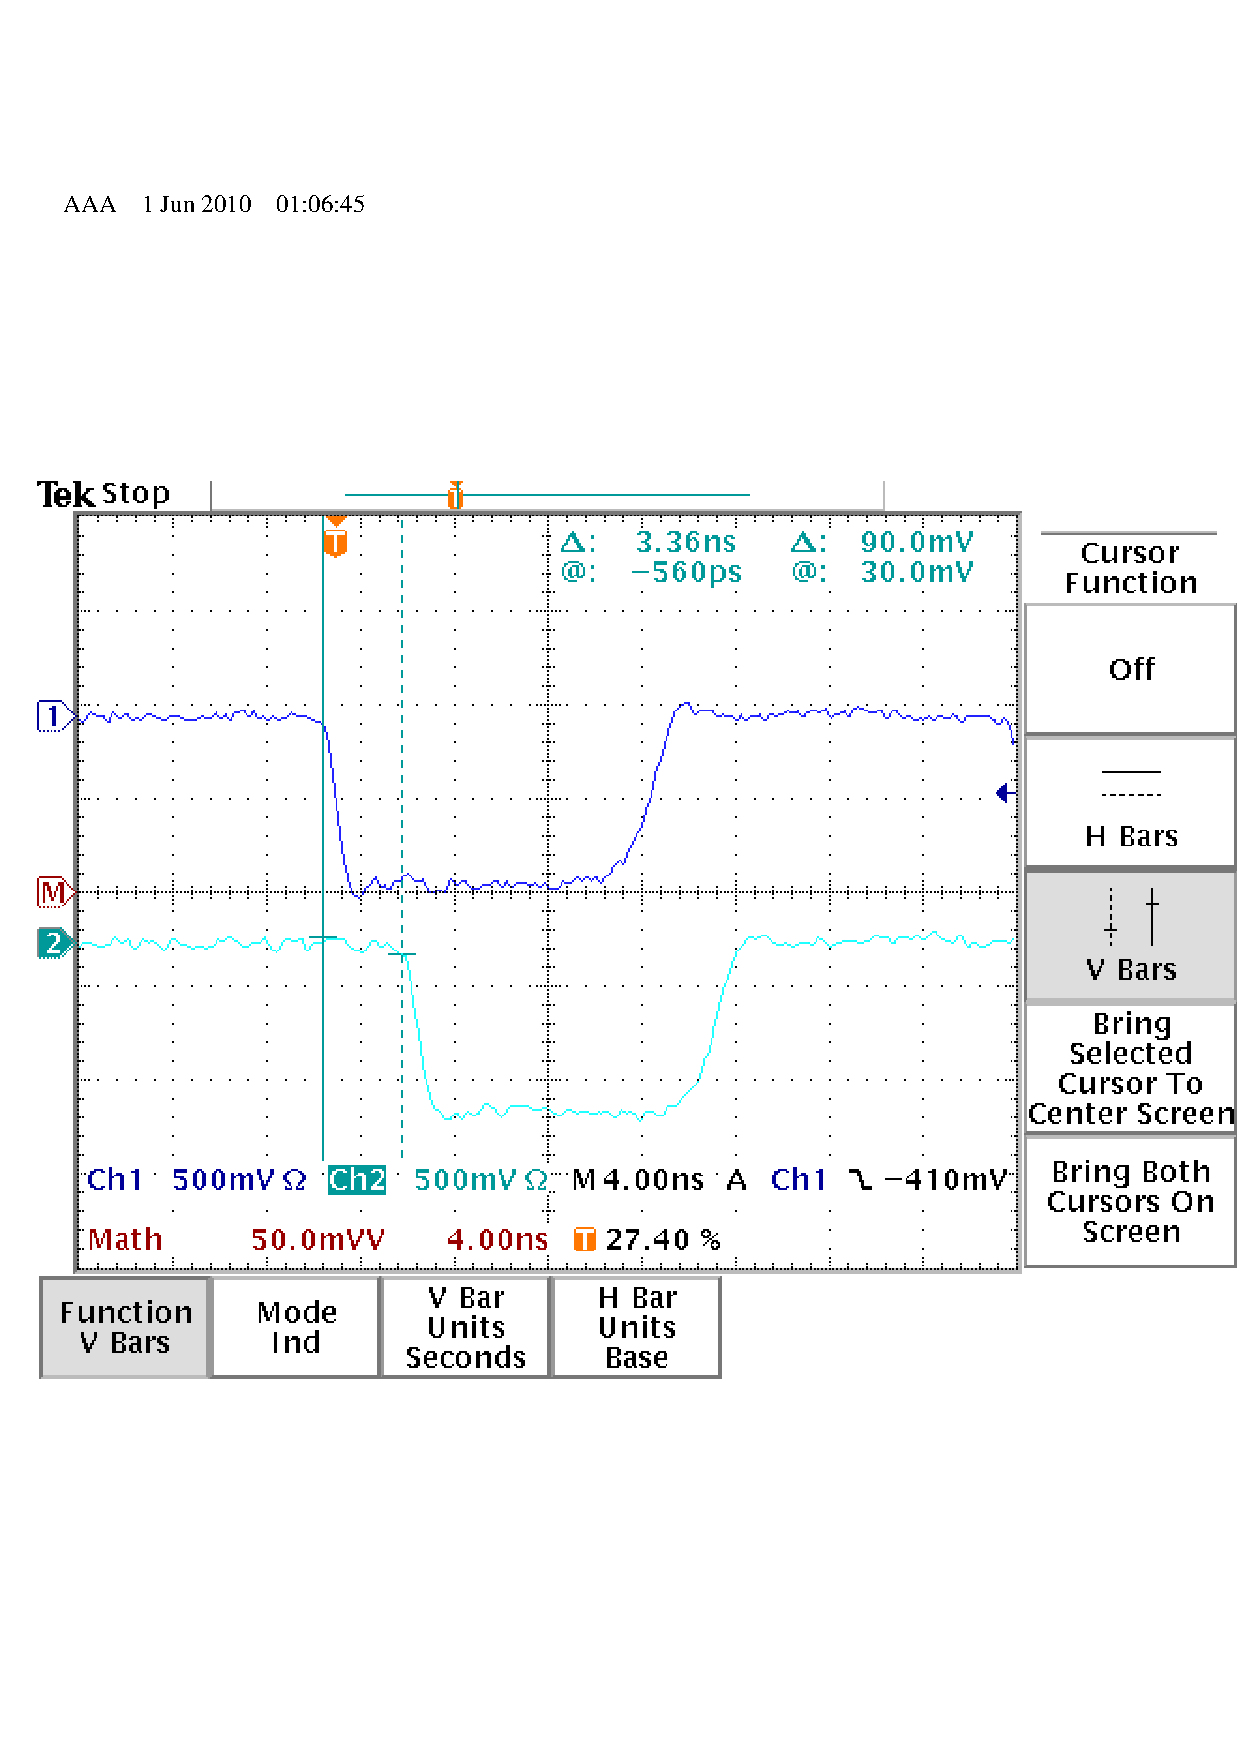
\includegraphics[width=1\columnwidth,keepaspectratio]{../tmp/TEK00010.pdf}
   \caption{Verzögerung in einer Koinzidenzeinheit}
   \label{fig:koinzidenz}
\end{figure}

Die Verzögerung wurde mit Hilfe der Positionsmarken, die zur Funktionalität des
Oszilloskops gehören, abgelesen, indem diese jeweils an den Beginn des Abfalls
der jeweiligen Kurve gefahren wurden. Die Differenz ist im oberen Bildteil in
der mit $\Delta:$ beginnenden Zeile abzulesen. Wir haben diese Messung sechs
mal durchgeführt. Die Zeitdifferenzen $t_i$ sind in \tref{diff} dargestellt.

\begin{table}[htbp]
\centering
% \setlength{\tabcolsep}{14pt}
\begin{tabular*}{0.95\columnwidth}{%
S[tabformat=1.2]%
S[tabformat=1.2]%
S[tabformat=1.2]%
S[tabformat=1.2]%
S[tabformat=1.2]%
S[tabformat=1.2]%
S[tabformat=2.1]%
}
\toprule
% daten aus ../data/TEK00006.pdf bis 12
{$t_1$} & {$t_2$} & {$t_3$} & {$t_4$} & {$t_5$} & {$t_6$} & {$t_7$}\\
\midrule
3,36 & 4,24 & 0,880 & 8,56 & 0,240 & 0,640 & 24,2\\
\bottomrule
\end{tabular*}
\caption{Messwerte der Verzögerungszeiten (angegeben in ns)}
\label{tab:diff}
\end{table}

Die Unsicherheiten der Zeiten liegen (je nach Messbereich) bei einem oder zwei
LSD (last significant digit). Wie man erkennen kann, schwanken die Zahlen
stark, was daran liegt, dass hier noch gar keine Ereignisselektion
stattgefunden hat und somit alle möglichen Events betrachtet wurden. Man kann
aber auch sehen, dass manche Zeitdifferenzen im Bereich von etwa
\SI{0,2}{\nano\second} liegen, also auf jeden Fall vernachlässigbar gegenüber
den Unsicherheiten der anderen Komponenten sind, zumal man davon ausgehen kann,
dass gerade diese Events diejenigen sind, die in Wirklichkeit gleichzeitig
stattfanden. Die Verzögerung wird also in diesem Bereich liegen und somit die
weitere Auswertung nicht beeinflussen.

\subsection{Bestimmung der Ereignisraten}

In diesem Versuchsteil wurden die Zählraten für verschiedene Kombinationen von
Photomultipliern und Szintillatoren gemessen.

\subsection{Ereignisraten für die einzelnen Photomultiplier}

Als erstes haben wir die in den einzelnen Photomultipliern auftretenden
Ereignisraten jeweils acht mal gemessen. Die resultierenden Mittelwerte der
Messwerte inkl. deren Fehler sind in \tref{pm_messwerte} zusammengetragen.

\begin{table}[htbp]
\centering
% \setlength{\tabcolsep}{14pt}
\begin{tabular*}{\columnwidth}{l|rrrrr}%
% S[tabformat=1.2]%
% S[tabformat=1.2]%
% S[tabformat=1.2]%
% S[tabformat=1.2]%
% S[tabformat=1.2]%
% S[tabformat=1.2]%
% }
\toprule
& {$N_1$} & {$N_2$} & {$N_3$} & {$N_4$} & {$N_5$}\\
\midrule
Rate & 1094 & 1878 & 1936 & 1178 & 1797\\
Fehler & 33 & 43 & 44 & 34 & 42\\
\bottomrule
\end{tabular*}
\caption{Mittelwerte der Ereignisraten $N_i$ (in \SI{1}{\per\second}) in den
Photomultipliern $PM_i$}
\label{tab:pm_messwerte}
\end{table}
Hierbei wurde angenommen, dass man die statistischen Fehler über einfaches
Radizieren ermitteln kann:
\begin{equation}
σ = \Delta N = \sqrt{N},
\end{equation}
was nur bei hinreichend großen Messwertanzahlen $N$ korrekt ist. Da $N$ bei uns
in der Größenordnung von 1000 liegt, sollte diese Annahme gerechtfertigt sein.
Eine Mittelwertbildung ist erlaubt, da man davon ausgehen kann, dass alle
Messungen statistisch unabhängig voneinander sind, aber den gleichen
physikalischen Prozess beschreiben.

Nun war zu untersuchen, wie stark die Effizienz abnimmt, wenn man in den
einzelnen Szintillationszählern eine Rechts-Links-Koinzidenz fordert. Dafür
haben wir eine entsprechende Logikschaltung aufgebaut, die diese zeitliche
Übereinstimmung überprüft. Auch hier haben wir immer acht mal gemessen; die
Mittelwerte sowie die Fehler können in \tref{SC2_SC3_koinzidenz} betrachtet
werden.

\begin{table}[htbp]
\centering
\begin{tabular*}{\columnwidth}{l|cc}
\toprule
& {SC2: $PM_2\wedge PM_4$} & SC3: $PM_3\wedge PM_5$\\
\midrule
Rate & 151 & 204\\
Fehler & 12 & 14\\
\bottomrule
\end{tabular*}
\caption{Mittelwerte der Ereignisraten (in \SI{1}{\per\second}) in den
Szintillationszählern SC2 und SC3}
\label{tab:SC2_SC3_koinzidenz}
\end{table}
Auch hier haben wir die Standardabweichung nach dem oben erwähnten Verfahren
bestimmt.

Wie man erkennen kann, nimmt die Zahl der Ereignisse deutlich ab. Der
Mittelwert der in den einzelnen Photomultipliern 2 und 4 bzw. 3 und 5 gemessenen
Raten wird im Folgenden angegeben, ebenso die Effizienz:
\begin{eqnarray}
MW_1 &\equiv& \frac{N_2+N_4}{2} = 1528\\
ε_1 &\equiv& \frac{N_{2\wedge4}}{V_1} = 0,099\\
MW_2 &\equiv& \frac{N_3+N_5}{2} = 1867\\
ε_2 &\equiv& \frac{N_{3\wedge5}}{V_2} = 0,109\\		%fehlerbetrachtung
\end{eqnarray}
Die Effizienz sinkt durch die neue Forderung auf etwa 10 bis 11 Prozent des
ursprünglichen Wertes. Dadurch wird sicherlich die zur Auswertung zur Verfügung
stehende Statistik verringert, aber dafür wird vor allem störender Hintergrund
ausselektiert. Der Hauptuntergrund entsteht in diesem Fall durch zufällig in
den Photomultipliern emittierte Elektronen, und da diese im Allgemeinen nicht
gleichzeitig in beiden zu einem Szintillationszähler gehörenden
Photomultipliern ausgelöst werden, ist die Koinzidenzforderung ein wirksamer
Filter gegen solche Effekte. Man kann somit relativ sicher sein, dass ein reales
Signal gemessen wurde (was aber noch kein Myonensignal sein muss; deren
Selektion erfolgt später.) Daher gleicht die resultierende Reinheit des Signals
den Nachteil der geringeren Statistik weit mehr als aus, sodass im Folgenden
für alle Szintillatoren eine solche Forderung gestellt wird.

Außerdem wurden die Raten in den einzelnen Szintillationszählern gemessen,
wobei weiterhin gefordert wird, dass die jeweils anderen Szintillatoren in
diesem Augenblick kein Ereignis detektieren. Die sich ergebenden Raten sind in
\tref{einzelne_szintillatoren} dargestellt.

\begin{table}[htbp]
\centering
\begin{tabular*}{0.8\columnwidth}{c|cc}
\toprule
& Rate & Fehler\\
\midrule
$SC_1 \neg SC_2 \neg SC_3$ & 1007 & 32\\
$\neg SC_1 \wedge SC_2 \neg SC_3$ & 199 & 14\\
$\neg SC_1 \neg SC_2 \wedge SC_3$ & 259 & 16\\
\bottomrule
\end{tabular*}
\caption{Mittelwerte der Ereignisraten (in \SI{1}{\per\second}) in den
Szintillationszählern $SC_i$}
\label{tab:einzelne_szintillatoren}
\end{table}

Wie man erkennen kann, ist die Rate in $SC_1$ deutlich größer als in den
anderen Szintillationszählern, was dadurch bedingt ist, dass in unserem
Experiment dieser Szintillator nur mit einem Photomultiplier ausgestattet war,
sodass hier das thermische Rauschen in diesem nicht herausgefiltert werden
konnte. 

Schließlich sollten die Raten untersucht werden, die sich ergeben, wenn man
verlangt, dass bestimmte Kombinationen von Szintillatoren gleichzeitig
ansprechen. Dies ist auch für die nachfolgenden Versuchsteile von Bedeutung, da
die Selektion der Myonenereignisse über solche Kombinationen erfolgt. Auch hier
haben wir für jede Kombination acht Messwerte aufgenommen, deren Mittelwerte
und statistische Fehler in \tref{sc_kombinationen} aufgeführt sind.

\begin{table}[htbp]
\centering
\begin{tabular*}{0.8\columnwidth}{r|cc}
\toprule
& Rate & Fehler\\
\midrule
$SC_1 \wedge SC_2$ & 20 & 1\\
$SC_1 \wedge SC_2 \wedge SC_3$ & 10 & 1\\
$SC_1 \wedge SC_2 \neg SC_3$ & 10 & 1\\
$SC_2 \wedge SC_3$ & 36 & 2\\
$SC_2 \vee SC_3$ & 948 & 31\\
\bottomrule
\end{tabular*}
\caption{Mittelwerte der Ereignisraten (in \SI{1}{\per\second}) in den
Szintillationszählern $SC_i$}
\label{tab:sc_kombinationen}
\end{table}

Da hier (abgesehen vom letzten Fall) schon wesentlich stärkere Kriterien erfüllt
werden mussten, sinkt die Zahl der gemessenen Ereignisse deutlich ab. Aus
diesem Grund haben wir bei den ersten vier Fällen 10 Sekunden lang gemessen,
und dann durch diese Zeit dividiert, um die angegebene Rate zu erhalten. Daher
ist hier die statistische Unsicherheit kleiner als die Wurzel des Mittelwerts.
Der letzte Fall hingegen ($SC_2 \vee SC_3$) verlangt nur, dass in einem der
beiden angegebenen Detektoren ein Teilchen registriert wird, und somit ist
klar, dass die Zahl der Ereignisse in der Größenordnung der Summe der Events in
den beiden einzelnen Szintillatoren (s. \tref{einzelne_szintillatoren}
$\rightarrow \sum_i SC_{i=1}^2 = 458 $) entspricht. Allerdings muss man
feststellen, 
dass die Ereigniszahl für die Kombination $SC_2 \vee SC_3$ mit einem Wert von
948 $\pm$ 31 ca. doppelt so groß ist wie die eben genannte Summe, was wir nicht
erwartet haben. Im Falle der Messung der Rate $SC_2 \vee SC_3$ sind zwar
abgesehen von den in der Summe betrachteten Ereignissen in den einzelnen
Szintillationszählern auch noch solche Ereignisse enthalten, die gleichzeitig
in beiden Szintillationszählern registriert werden konnten, aber wir gehen
davon aus, dass diese Events wesentlich seltener als die nur in einem
Szintillator detektierten sind, weil diese Forderung nur Teilchen zulässt, die
sehr schnell sind und in eine geeignete Richtung fliegen. Der Faktor zwei ist
darüber also nicht erklärbar. Man muss also davon ausgehen, dass bei der
Messung ein Fehler unterlaufen ist, sodass dieses eine Ergebnis nicht zur
Einschätzung der Hintergrundrate verwendbar ist.

\subsection{Signalbetrachtung}
Zu allen im vorigen Abschnitt betrachteten Kombinationen von Photomultipliern
bzw. Szintillationszählern wurde exemplarisch ein Bild aufgezeichnet. Alle
Bilder sind im Anhang unter \ref{sec:plots} zu finden.

Zunächst haben wir die Signalformen der einzelnen Photomultiplier in \fref{PMs}
dargestellt. Man kann gut erkennen, dass alle Photomultiplier annähernd das
gleiche, gaußförmige Signalprofil aussenden, was auch zu erwarten war. Da wir
den Trigger auf den angezeigten Kanal eingestellt haben, kann man auch nur einen
einzelnen (negativen) Peak sehen.

In \fref{zeitdifferenzen} kann man die Zeitdifferenzen erkennen, die sich in
den Koinzidenzschaltungen aufgrund von Signallaufzeiten und der verarbeitenden
Logikelemente aus einem an sich (annähernd) gleichzeitig in beiden Multipliern
stattfindenden Ereignissen ergibt. Da wir immer auf Channel 1 triggern ließen
und keine Forderung an die Reihenfolge der Signale stellen, kommt es vor, dass
auch negative Werte gemessen werden, aber das Oszilloskop macht daraus von sich
aus bereits positive Zahlen, sodass wir uns über die Vorzeichen keine Gedanken
mehr machen müssen. Die aus den Bildern abgelesenen Zeitverzögerungen wurden in
\tref{diff} bereits aufgelistet.